\documentclass[spanish, fleqn]{article}
\usepackage[spanish]{babel}
\usepackage[utf8]{inputenc}
\usepackage{amsmath}
\usepackage{amsfonts,txfonts}
\usepackage{mathrsfs}
\usepackage[colorlinks, urlcolor=blue]{hyperref}
\usepackage{fourier}
\usepackage[top = 2.5cm, bottom = 2cm, left = 2cm, right = 2cm]{geometry}
\usepackage{graphicx}




\title{\textsc{Elementos de Análisis para Computación e Informática} \\
	\textsc{Examen Final}}

\author{Martín Villanueva}
\date{23 de Mayo 2016}

\begin{document}
\maketitle


\section*{\textsc{Tareas}}


\begin{description}

	\item[\textsc{Tarea 1.}] Sean $(X , \sigma)$ y $(X, \sigma')$ espacios métricos y quasimétricos respectivamente. Denotemos a la topología generada/inducida por $\sigma$ por:
	\begin{align*}
		\mathcal{F} = \{ A \subset X: \ A \ \text{es un abierto, i.e:} \ \ \forall x \in A, \ \exists \delta>0: \ B_{\sigma}(x,\delta) \subset A \}
	\end{align*}
	donde adicionalmente sabemos que una base para esta topología es:
	\begin{align*}
		B = \{ B_{\sigma}(x, \sigma): \ x \in X, \ \delta \ \in \mathbb{R}_{0}^{+}  \}
	\end{align*}
	y también consideremos la siguiente \textit{posible} base para dicha topología:
	\begin{align*}
		B' = \{ B_{\sigma'}(x,\delta): \ x \in X, \ \delta \ \in  \mathbb{R}_{0}^{+} \cup \{ \infty \} \}
	\end{align*}
	se puede ver claramente que $B \subset B'$, pues $B'$ contiene los mismos miembros que $B$, más las bolas de radio infinito (\textit{que abarcan todo el espacio!}). Además como $B$ es una base para $\mathcal{F}$, cualquier abierto $\in \mathcal{F}$ puede escribirse como una reunión de miembros de $B$.

	Sea $\mathcal{A}$ un conjunto indexador (no necesariamente contable, ni finito), entonces cualquier reunión de bolas \newline $ \bigcup_{\alpha \in \mathcal{A}} B_{\alpha}  \ (B_{\alpha} \in B)$, puede formarse también con miembros de $B'$, pues $B \subset B'$. 
	Consideremos ahora reuniones sobre $B'$. Si entre los miembros no hay bolas de radio infinito, el resultado es análogo 
	al anterior. Consideremos entonces el caso de una reunión con al menos una bola de radio infinito $B_{\sigma'}(x_0, \infty)$:
	\begin{align*}
		\bigcup_{\alpha \in \mathcal{A}} B_{\alpha} \ (B_{\alpha} \in B') = B_{\sigma'}(x_0, \infty)
	\end{align*}
	tal resultado puede obtenerse por reuniones de miembros en $B$ como sigue:
	\begin{align*}
		\bigcup_{\delta > 0} B_{\sigma}(x_0, \delta)
	\end{align*}

	Luego, hemos probado que cada reunión de miembros en una base, puede formarse con los miembros de la otra (y viceversa). Por lo tanto ambas son bases de $\mathcal{F}$, y entonces $\sigma$ y $\sigma'$ generan/inducen la misma topología.




	\item[\textsc{Tarea 2.}]




	\item[\textsc{Tarea 3.}]




	\item[\textsc{Tarea 4.}] Veamos cada punto separadamente:
	\begin{enumerate}
		\item $\displaystyle \int_{\mathbb{R}} |\chi_{[-1,1]}(t)|\ dt = \int_{-1}^{1} |1| dt = 2 < \infty$, por lo tanto $\chi_{[-1,1]} \in L^1$.
		\item $\displaystyle \widehat{\chi_{[-1,1]}(t)} = \int_{\mathbb{R}} \chi_{[-1,1]}(t) e^{-2 \pi i \omega t} dt = \int_{-1}^{1} e^{-2 \pi i \omega t} dt$. Haciendo uso de la identidad de Euler:
		\begin{align*}
			\int_{-1}^{1} e^{i (-2 \pi \omega t)} dt = \int_{-1}^{1} \cos(-2 \pi \omega t) + i \sin(-2 \pi \omega t) dt
		\end{align*}
		tomando en cuenta la paridad de las funciones (\textit{y que la integral de una función impar en un intervalo simétrico es nula}):
		\begin{align*}
			\ldots = \int_{-1}^{1} \cos(2 \pi \omega t) dt - i \underbrace{\int_{-1}^{1} \sin(2 \pi \omega t) dt]}_{= 0 \ \text{por imparidad}} = \frac{\sin(2 \pi \omega t)}{2 \pi \omega} \bigg|_{-1}^{1} = \frac{\sin(2 \pi \omega)}{\pi \omega}
		\end{align*}
		\item

	\end{enumerate}En




	\item[\textsc{Tarea 5.}] Veamos por partes:
	\begin{enumerate}
		\item Denotemos como $\displaystyle f(t)=e^{-t^2}$ y $\displaystyle g(t)=(1+t^2)^{-1}$. En primer lugar, es fácil notar que las derivadas de $f(t)$ son la misma función multiplicadas por un polinomio (\textit{regla de la cadena}). Cada nueva derivada aumenta en un grado el grado del polinomio respectivo, pues la derivada del exponente es $-2t$.
		Luego se puede escribir $f^{(n)}(t)=f(t)P_n(t)$, con $P_n$ el polinomio de grado $n$ respectivo. Entonces:
		\begin{align*}
			\lim_{|t|\rightarrow \infty} t^p D^q f(t) = \lim_{|t|\rightarrow \infty} t^p P_q(t) f(t) = \lim_{|t|\rightarrow \infty} \widehat{P}_{p+q}(t) f(t) = \lim_{|t|\rightarrow \infty} \frac{\widehat{P}_{p+q}(t)}{e^{t^2}} = 0 \ \ \ \forall \ p,q \in \mathbb{N}_0,
		\end{align*}
		lo último debido a que la exponencial crece más rápido que cualquier polinomio en $t \rightarrow \infty$. En segundo lugar, para probar que $g \notin \mathcal{C}^{\infty}(\mathbb{R},\mathbb{C})$, basta mostrar que existe alguna combinación de $p,q \in \mathbb{N}_0$ tales que $t^p D^q g(t) \rightarrow 0$ no se satisface. Veamos para $p=3$ y $q=1$:
		\begin{align*}
			\lim_{|t|\rightarrow \infty} \frac{t^3}{1+t^2} \rightarrow \infty,
		\end{align*}
		lo que completa la demostración.

		\item

		\item

		\item
	\end{enumerate}




	\item[\textsc{Tarea 6.}]



 
	\item[\textsc{Tarea 7.}] Se listan a continuación algunos ejemplos de funciones $f \in \mathcal{C}_{C}^{\infty}(\mathbb{R},\mathbb{C})$ (la extensión a varias variables se muestra a continuación):
	\begin{enumerate}
		\item Un ejemplo clásico es la función \textit{bump}, definida como:
		\begin{align*}
		\psi(x) =
		\begin{cases}
		e^{\frac{1}{x^2-1}} & |x|<1 \\
		0 & |x|>= 1,
		\end{cases}	
		\end{align*}
		cuya grafica se ve en Figura \ref{fig:cbump}. Esta puede ser fácilmente extendida a otros invervalos de compacidad:
		\begin{align*}
		\widehat{\psi}(x) =
		\begin{cases}
		e^{\frac{1}{(x-a)^2-1}} & |x|<r \\
		0 & |x|>= r,
		\end{cases}	
		\end{align*}
		que tiene soporte compacto en $[a-r, a+r]$ con $a,r \in \mathbb{R}$. 

	\begin{figure}[htpb!]
	\centering
	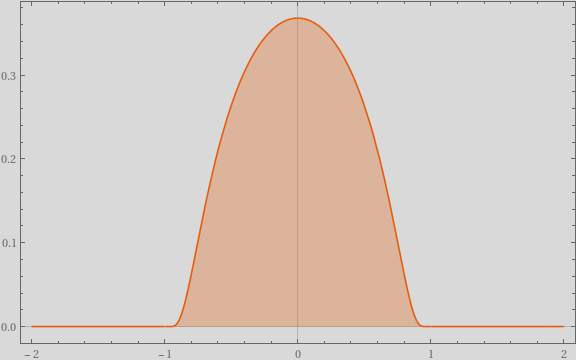
\includegraphics[width=10cm]{bump}
	\caption{Gráfico de función \textit{bump} clásica.}
	\label{fig:cbump}
	\end{figure}

	\item Otra construcción interesante considera a la función $\displaystyle f(x) = e^{\frac{-1}{x}}$, cuya ``gracia'' es que está en $\mathcal{C}^{\infty}$ y $f(0)=0$. Con esta es posible definir:
	\begin{align}
		\phi(x) = \frac{f(x)}{f(x)-f(1-x)}
	\label{eq:trick}
	\end{align}
	la cual tambien pertenece a $\mathcal{C}^{\infty}$, pero ademas $\phi(0)=0$ y $\phi(1)=1$. Entonces una función de soporte compacto se puede construir como sigue:
	\begin{align*}
		\psi(x) =
		\begin{cases}
		0 & x \leq 0 \\
		\phi(x) & 0 < x <1 \\
		1 & 1 \leq x \leq a \\
		\phi(-(x-[a+1])) & a < x < a+1 \\
		0 & x \geq a+1
		\end{cases}	
	\end{align*}
	donde $a \in \mathbb{R}\ (> 1)$. Que básicamente consiste en poner la ``copia'' invertida de $\phi$ (respecto al eje $y$) y trasladada a la derecha en $a+1$, y definiendo el valor de la función en el intervalo intermedio $[1,a]$ como $1$ para asegurar la continuidad. En la Figura \ref{fig:const} se muestra esta contrucción con $a=2$.
	\begin{figure}[htpb!]
	\centering
	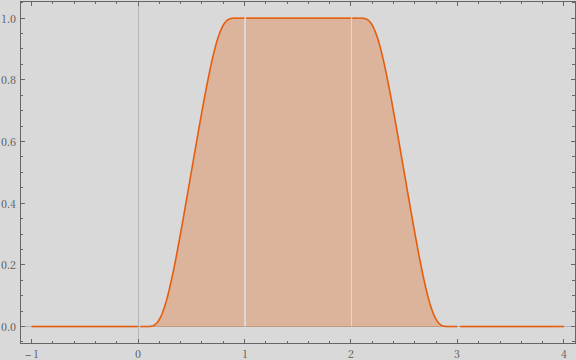
\includegraphics[width=10cm]{construction}
	\caption{Construcción de función de soporte compacto.}
	\label{fig:const}
	\end{figure}
	
	Notar que la misma construcción puede realizarse siguiendo el mismo procedimiento y usando (\ref{eq:trick}), pero con
	alguna otra función $f$ que cumpla $f \in \mathcal{C}^{\infty}$ y $f(0)=0$.

	\end{enumerate}

	Por último, dada una función $\psi \in \mathcal{C}_{C}^{\infty}(\mathbb{R},\mathbb{C})$ con soporte $[a,b] \ \text{y} \ a,b \in \mathbb{R}$, esta puede ser fácilmente extendida a una función $\in \mathcal{C}_{C}^{\infty}(\mathbb{R}^n,\mathbb{C})$, bajo la siguiente construcción:
	\begin{align}
	\Phi(x_1,x_2,\ldots,x_n) = \psi(x_1)\ \psi(x_2)\ \cdots \ \psi(x_n),
	\label{eq:ndbump}
	\end{align}
	cuyo soporte compacto es $[a,b]\times \stackrel{n-2 \text{ veces}}{\ldots} \times [a,b]=[a,b]^n$. En la Figura \ref{fig:3dbump} se muestra tal construcción para la función \textit{bump} clásica en dos variables.
	
	\begin{figure}[htpb!]
	\centering
	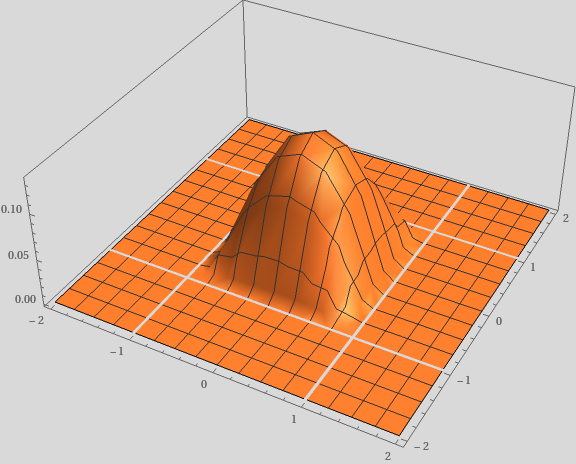
\includegraphics[width=10cm]{3dbump}
	\caption{Gráfico de función \textit{bump} clásica en dos variables.}
	\label{fig:3dbump}
	\end{figure}



	\item[\textsc{Tarea 8.}] Sea $f \in \mathcal{C}_{\downarrow}^{\infty}(\mathbb{R},\mathbb{C})$ una función con soporte compacto $\text{supp}(f) \subset [a,b] \subset [0,T]$ ($0<a<b<T$), con la respectiva prolongación periódica (de periodo $T$)
	\begin{align}
	 	g(x) = \sum_{n \in \mathbb{Z}} f(x - n T), \ \ \ \ x \in \mathbb{R}.
	 	\label{eq:prolongacion}
	\end{align} Considerando la norma uniforme $||f||_{\infty} := \sup_{x \in \mathbb{R}} |f(x)|$. Como ya probamos anteriormente (Weierstrass):
	\begin{align*}
		f \in \mathcal{C}_{\downarrow}^{\infty}(\mathbb{R},\mathbb{C}) \Rightarrow 0 \leq ||f||_{\infty} < \infty.
	\end{align*}
	Debido a la construcción de la prologación periódica (\ref{eq:prolongacion}), se sabe que no existen traslapes entre
	las \textit{copias} de $f$ en los distintos periodos. Entonces:
	\begin{align*}
		||g||_{\infty} = \sup_{x \in \mathbb{R}} |g(x)| = \sup_{x \in \mathbb{R}} \left|\sum_{n \in \mathbb{Z}} f(x - n T)\right| \stackrel{(\#)}{=} \sup_{x \in \mathbb{R}} |f(x-nT)|\ \ (\forall n \in \mathbb{Z})= \sup_{x \in \mathbb{R}} |f(x)| = ||f||_{\infty} < \infty 
	\end{align*}
	donde $(\#)$ es posible, pues como se hizo notar, todas las copias de $f$ son iguales y sin traslapes. Puesto que $||g||_{\infty} < \infty$, se comprueba entonces la convergencie de la serie.




	\item[\textsc{Tarea 9.}] 

\end{description}


\section*{\textsc{Referencias}}



\end{document}
